%package list
\documentclass{article}
\usepackage[top=3cm, bottom=3cm, outer=3cm, inner=3cm]{geometry}
\usepackage{multicol}
\usepackage{graphicx}
\usepackage{url}
%\usepackage{cite}
\usepackage{hyperref}
\usepackage{array}
%\usepackage{multicol}
\newcolumntype{x}[1]{>{\centering\arraybackslash\hspace{0pt}}p{#1}}
\usepackage{natbib}
\usepackage{pdfpages}
\usepackage{multirow}
\usepackage[normalem]{ulem}
\useunder{\uline}{\ul}{}
\usepackage{svg}
\usepackage{xcolor}
\usepackage{listings}
\lstdefinestyle{ascii-tree}{
    literate={├}{|}1 {─}{--}1 {└}{+}1 
  }
\lstset{basicstyle=\ttfamily,
  showstringspaces=false,
  commentstyle=\color{red},
  keywordstyle=\color{blue}
}
%\usepackage{booktabs}
\usepackage{caption}
\usepackage{subcaption}
\usepackage{float}
\usepackage{array}

\newcolumntype{M}[1]{>{\centering\arraybackslash}m{#1}}
\newcolumntype{N}{@{}m{0pt}@{}}


%%%%%%%%%%%%%%%%%%%%%%%%%%%%%%%%%%%%%%%%%%%%%%%%%%%%%%%%%%%%%%%%%%%%%%%%%%%%
%%%%%%%%%%%%%%%%%%%%%%%%%%%%%%%%%%%%%%%%%%%%%%%%%%%%%%%%%%%%%%%%%%%%%%%%%%%%
\newcommand{\itemEmail}{adelgadoal@unsa.edu.pe}
\newcommand{\itemStudent}{Andre David Delgado Allpan}
\newcommand{\itemCourse}{Programación web}
\newcommand{\itemCourseCode}{20231001}
\newcommand{\itemSemester}{III}
\newcommand{\itemUniversity}{Universidad Nacional de San Agustín de Arequipa}
\newcommand{\itemFaculty}{Facultad de Ingeniería de Producción y Servicios}
\newcommand{\itemDepartment}{Departamento Académico de Ingeniería de Sistemas e Informática}
\newcommand{\itemSchool}{Escuela Profesional de Ingeniería de Sistemas}
\newcommand{\itemAcademic}{2023 - A}
\newcommand{\itemInput}{Del 2 Junio 2023}
\newcommand{\itemOutput}{Al 6 Junio 2023}
\newcommand{\itemPracticeNumber}{04}
\newcommand{\itemTheme}{Python}
%%%%%%%%%%%%%%%%%%%%%%%%%%%%%%%%%%%%%%%%%%%%%%%%%%%%%%%%%%%%%%%%%%%%%%%%%%%%
%%%%%%%%%%%%%%%%%%%%%%%%%%%%%%%%%%%%%%%%%%%%%%%%%%%%%%%%%%%%%%%%%%%%%%%%%%%%

\usepackage[english,spanish]{babel}
\usepackage[utf8]{inputenc}
\AtBeginDocument{\selectlanguage{spanish}}
\renewcommand{\figurename}{Figura}
\renewcommand{\refname}{Referencias}
\renewcommand{\tablename}{Tabla} %esto no funciona cuando se usa babel
\AtBeginDocument{%
	\renewcommand\tablename{Tabla}
}

\usepackage{fancyhdr}
\pagestyle{fancy}
\fancyhf{}
\setlength{\headheight}{30pt}
\renewcommand{\headrulewidth}{1pt}
\renewcommand{\footrulewidth}{1pt}
\fancyhead[L]{\raisebox{-0.2\height}{
\includegraphics[width=3cm]{img/logo_episunsa.png}}}
\fancyhead[C]{\fontsize{7}{7}\selectfont	\itemUniversity \\ \itemFaculty \\ \itemDepartment \\ \itemSchool \\ \textbf{\itemCourse}}
\fancyhead[R]{\raisebox{-0.2\height}{
\includegraphics[width=1.2cm]{img/logo_abet}}}
\fancyfoot[L]{Estudiante Andre Delgado Allpan}
\fancyfoot[C]{\itemCourse}
\fancyfoot[R]{Página \thepage}

% para el codigo fuente
\usepackage{listings}
\usepackage{color, colortbl}
\definecolor{dkgreen}{rgb}{0,0.6,0}
\definecolor{gray}{rgb}{0.5,0.5,0.5}
\definecolor{mauve}{rgb}{0.58,0,0.82}
\definecolor{codebackground}{rgb}{0.95, 0.95, 0.92}
\definecolor{tablebackground}{rgb}{0.8, 0, 0}

\lstset{frame=tb,
	language=bash,
	aboveskip=3mm,
	belowskip=3mm,
	showstringspaces=false,
	columns=flexible,
	basicstyle={\small\ttfamily},
	numbers=none,
	numberstyle=\tiny\color{gray},
	keywordstyle=\color{blue},
	commentstyle=\color{dkgreen},
	stringstyle=\color{mauve},
	breaklines=true,
	breakatwhitespace=true,
	tabsize=3,
	backgroundcolor= \color{codebackground},
}

\begin{document}
	
	\vspace*{10px}
	
	\begin{center}	
		\fontsize{17}{17} \textbf{ Informe de Laboratorio \itemPracticeNumber}
	\end{center}
	\centerline{\textbf{\Large Tema: \itemTheme}}
	%\vspace*{0.5cm}	

	\begin{flushright}
		\begin{tabular}{|M{2.5cm}|N|}
			\hline 
			\rowcolor{tablebackground}
			\color{white} \textbf{Nota}  \\
			\hline 
			     \\[30pt]
			\hline 			
		\end{tabular}
	\end{flushright}	

	\begin{table}[H]
		\begin{tabular}{|x{4.7cm}|x{4.8cm}|x{4.8cm}|}
			\hline 
			\rowcolor{tablebackground}
			\color{white} \textbf{Estudiante} & \color{white}\textbf{Escuela}  & \color{white}\textbf{Asignatura}   \\
			\hline 
			{\itemStudent \par \itemEmail} & \itemSchool & {\itemCourse \par Semestre: \itemSemester \par Código: \itemCourseCode}     \\
			\hline 			
		\end{tabular}
	\end{table}		
	
	\begin{table}[H]
		\begin{tabular}{|x{4.7cm}|x{4.8cm}|x{4.8cm}|}
			\hline 
			\rowcolor{tablebackground}
			\color{white}\textbf{Laboratorio} & \color{white}\textbf{Tema}  & \color{white}\textbf{Duración}   \\
			\hline 
			\itemPracticeNumber & \itemTheme & 04 horas   \\
			\hline 
		\end{tabular}
	\end{table}
	
	\begin{table}[H]
		\begin{tabular}{|x{4.7cm}|x{4.8cm}|x{4.8cm}|}
			\hline 
			\rowcolor{tablebackground}
			\color{white}\textbf{Semestre académico} & \color{white}\textbf{Fecha de inicio}  & \color{white}\textbf{Fecha de entrega}   \\
			\hline 
			\itemAcademic & \itemInput &  \itemOutput  \\
			\hline 
		\end{tabular}
	\end{table}
	
	\section{Tarea}
	\begin{itemize}		
		\item General: Diseña responsablemente aplicaciones web, sus componentes o procesos para satisfacer necesidades dentro de restricciones realistas: económicas, medio ambientales, sociales,
políticas, éticas, de salud, de seguridad, manufacturación y sostenibilidad.
		\item Específica: Construye responsablemente soluciones con tecnología web siguiendo un proceso adecuado llevando a cabo las pruebas ajustada a los recursos disponibles del cliente.
		\item Específica: C.p. Aplica de forma flexible técnicas, métodos, principios, normas, estándares y herramientas del desarrollo web necesarias para la construcción de aplicaciones web e implementación de estos sistemas en una organización.
	\end{itemize}
	
	\section{Resultados del estudiante}
	\begin{itemize}
		\item RE. 2: La capacidad de aplicar diseño de ingeniería para producir soluciones a problemas y diseñar sistemas, componentes o procesos para satisfacer necesidades específicas dentro de consideraciones realistas en los aspectos de salud pública, seguridad y bienestar; factores globales, culturales, sociales, económicos y ambientales.
		\item RE. 8: La capacidad de crear, seleccionar y utilizar técnicas, habilidades, recursos y herramientas modernas de ingeniería y tecnologías de la información, incluyendo la predicción y el modelamiento, con una comprensión de las limitaciones.
	\end{itemize}
		
	\section{Equipos, materiales y temas utilizados}
	\begin{itemize}
		\item Sistema Operativo Ubuntu GNU Linux 23 lunar 64 bits Kernell 6.2.
		\item VIM 9.0.
		\item OpenJDK 64-Bits 17.0.7.
		\item Git 2.39.2.
		\item Cuenta en GitHub con el correo institucional.
		\item Programación Orientada a Objetos.
		\item Algoritmo de ordenamiento por inserción	
	\end{itemize}
	
	\section{URL de Repositorio Github}
	\begin{itemize}
		\item URL del Repositorio GitHub para clonar o recuperar.
		\item \url{https://github.com/rescobedoq/pw2.git}
		\item URL para el laboratorio 01 en el Repositorio GitHub.
		\item \url{https://github.com/andre98652/pweb-lab4.git}
	\end{itemize}
	
	\section{Marco Teórico}
	
	\subsection{Python}
	\begin{itemize}	
		\item Python es un lenguaje de programación interpretado no fuertemente tipado.
		
	\end{itemize}	
	\subsection{Instalación en GNU/Linux}
	\begin{itemize}	
		\item Para instalar Python 3 en cualquier distribución GNU/Linux use sus mismos repositorios.
		\item Por ejemplo en sistemas operativos compatibles con GNU/Linux Debian use alguno de los dos comandos siguientes:
	\end{itemize}	
	\begin{lstlisting}[language=bash,caption={Instalar Python en GNU/Linux Debian}][H]
		# apt-get install python3
	\end{lstlisting}
	\begin{lstlisting}[language=bash,caption={Instalar Python en GNU/Linux Ubuntu}][H]
		$ sudo apt-get install python3
	\end{lstlisting}	
	
	
	\subsection{Instalación en MS Windows}
	
	
	\begin{itemize}	
		\item Para descargar Python compatible con sistemas operativos MS Windows utilice alguno de los instaladores de: \url{https://www.python.org/downloads/windows/}
		\item Descargar e instalar en sistemas operativos MS Windows, por lo general es muy sencillo. Además si usted es un usuario nativo de windows este proceso será casi intuitivo. No tenga miedo de instalar estos programas todo es software libre, asi que no necesitará parches o cracks. :)
	\end{itemize}
	
	\subsection{Instalación en MS MacOS}
	
	\begin{itemize}	
		\item Para instalar Python 3 en sistemas operativos MacOS puede descargar el instalador desde: \url{https://www.python.org/downloads/macos/} o usar brew:
	\end{itemize}
	
	\begin{lstlisting}[language=bash,caption={Instalar Python en MacOS}][H]
		$ brew install python
	\end{lstlisting}
	
	\subsection{Comprobar presencia y versión de Python}
	\begin{itemize}
		\item Debe comprobar que la instalación y el reconocimiento del compilador ya estan presentes en su sistema operativo:
	\end{itemize}
	
	\begin{lstlisting}[language=bash,caption={Verificando presencia y versión de Python}][H]
		$ python3 --version
	\end{lstlisting}
	
	\begin{itemize}
		\item Usted debería obtener como salida la versión que tiene instalada.
	\end{itemize}
	\begin{lstlisting}[language=bash,caption={Verificando presencia y versión de Python}][H]
		Python 3.11.2
	\end{lstlisting}
	
	\subsection{Hola mundo}
	
	\begin{itemize}
		\item Cree su primer ejercicio \textbf{helloworld.py}
	\end{itemize}
	\begin{lstlisting}[language=bash,caption={Creando el archivo helloworld.py}][H]
		$ vim helloworld.py
	\end{lstlisting}
	\begin{lstlisting}[language=bash,caption={helloworld.py}][H]
		print("Hello World!")
	\end{lstlisting}
	\begin{itemize}
		\item Para ejecutar su script \textbf{helloworld.py} ejecute el siguiente comando:
	\end{itemize}
	\begin{lstlisting}[language=bash,caption={Ejecutando el script helloworld.py}][H]
		$ python3 helloworld.py
	\end{lstlisting}
	
	\subsection{Comentarios en Python}
	\begin{itemize}
		\item Los comentarios de Python solo se aplican por cada línea.
		\item Pero usted puede utilizar varias técnicas para comentar en el editor de Vim
	\end{itemize}
	
	\begin{lstlisting}[language=bash,caption={Comentar rango de 	líneas 5-10}][H]
		:3,5s/^/#
	\end{lstlisting}
	\begin{lstlisting}[language=bash,caption={Comentar todas las líneas que tengan la palabra print}][H]
		:g/print/s/^/#
	\end{lstlisting}
	
	\subsection{Virtual Environment}
	\begin{itemize}
		\item La reutilización de código fuente (paquetes, librerias, plugins, etc.) de terceros nos permite construir software más complejo, sobre todo con menos tiempo.
		\item En NodeJS se usaban paquetes instalados en el directorio de trabajo y no de manera global,registrando estos paquetes en sus versiones en el archivo package.json.
		\item Por eso este modo de trabajo nos permite tener distintos proyectos con distintas bibliotecas, de distintas versiones, en la misma máquina, sin que existan conflictos.
		\item Para compartir el proyecto se debe compartir el archivo package.json y luego llamar a ”npm install”para instalar las bibliotecas adecuadas para el proyecto.
		\item Java usa ant y maven, junto con archivos xml para realizar estas tareas.
		\item Python tiene \textbf{virtualenv}, para crear este espacio de trabajo.
		\item Python utiliza el manejador de paquetes pip.
	\end{itemize}
	
	\subsection{Pip}
	\begin{itemize}
		\item Instalemos pip, una herramienta que instalará y administrará los paquetes de programación que queramos usar en nuestros proyectos de desarrollo.
	\end{itemize}
	\begin{lstlisting}[language=bash,caption={Instalación de pip}][H]
		$ sudo apt-get install -y python3-pip
	\end{lstlisting}
	
	\subsection{Garantizando posibilidades para trabajar con entornos virtuales}
	\begin{itemize}
		\item Paquetes y herramientas de desarrollo más para instalar para garantizar que tengamos una configuración sólida para nuestro entorno de programación.
	\end{itemize}
	\begin{lstlisting}[language=bash,caption={Instalaciones previas para entorno virtual}][H]
		$ sudo apt-get install build-essential libssl-dev libffi-dev python3-dev
	\end{lstlisting}
	
	\subsection{Instalación de paquetes para crear entornos virtuales}
	\begin{itemize}
		\item Los entornos virtuales permiten tener un espacio aislado en los proyectos Python.
		\item Garantizando que cada proyecto pueda tener su propio conjunto de dependencias que no interrumpirán a otros proyectos.
		\item Manejando diferentes versiones de los paquetes. Esto es especialmente importante cuando se trabaja con paquetes de terceros.
		\item Puede varios entornos de programación.
		\item Cada entorno es un directorio en la que se ubicarán sus scripts.
		\item Usaremos el módulo venv, que es parte de la biblioteca estándar de Python.
		\item Instalemos venv escribiendo:
	\end{itemize}
	\begin{lstlisting}[language=bash,caption={Instalación del entorno virtual}][H]
		$ sudo apt-get install -y python3-venv
		$ sudo apt-get install python3-virtualenv
	\end{lstlisting}
	
	\subsection{Crear un directorio para entorno virtual}
	\begin{itemize}
		\item Para crear un ambiente elija en qué directorio se va a crear el entorno virtual.
	\end{itemize}
	\begin{lstlisting}[language=bash,caption={Creando directorio para entorno virtual}][H]
		$ mkdir -p $HOME/rescobedoq/pw2-lab-c-23a/lab04/my_env
	\end{lstlisting}
	
	\subsection{Crear entorno virtual en un directorio}
	\begin{itemize}
		\item En este directorio crear un entorno virtual ejecutando el siguiente comando:
	\end{itemize}
	\begin{lstlisting}[language=bash,caption={Creando entorno virtual}][H]
		$ cd $HOME/rescobedoq/pw2-lab-c-23a/lab04/my_env
		$ virtualenv -p python3 .
	\end{lstlisting}
	
	\subsection{Estructura de un entorno virtual}
	\begin{itemize}
		\item Estudie la estructura del entorno virtual.
		\item Dentro del directorio para el entorno virtual se debió crear un subdirectorio src/ con el siguiente contenido:
	\end{itemize}
	\begin{lstlisting}[language=bash,caption={Creando entorno virtual}][H]
		$ cd $HOME/rescobedoq/pw2-lab-c-23a/lab04/my_env
		$ virtualenv -p python3 .
	\end{lstlisting}
	\begin{lstlisting}[style=ascii-tree]
.
|--- bin
| |--- activate
| |--- activate.csh
| |--- activate.fish
| |--- activate.nu
| |--- activate.ps1
| |--- activate_this.py
| |--- deactivate.nu
| |--- pip
| |--- pip-3.9
| |--- pip3
| |--- pip3.9
| |--- python -> /usr/local/opt/python@3.9/bin/python3.9
| |--- python3 -> python
| |--- python3.9 -> python
| |--- wheel
| |--- wheel-3.9
| |--- wheel3
| |--- wheel3.9
|--- lib
| |--- python3.9
|--- pyvenv.cfg
|--- text.txt
3 directories, 20 files
	\end{lstlisting} 
	
	\subsection{Activando entorno virtual}
	\begin{itemize}
		\item En el directorio de trabajo active el entorno virtual ejecutando el script \textbf{activate}:
	\end{itemize}
	\begin{lstlisting}[language=bash,caption={Activando entorno virtual}][H]
		$ cd $HOME/rescobedoq/pw2-lab-c-23a/lab04/exercises/
		$ source ./../my_env/bin/activate
		(my_env) user@localhost:$
	\end{lstlisting}
	
	\subsection{Trabajando dentro del entorno virtual}
	\begin{itemize}
		\item Cree el \textbf{Hola Mundo} con su entorno virtual activado.
		\item Al finalizar todos sus ejercicios, no olvide de desactivar el entorno virtual.
	\end{itemize}
	\begin{lstlisting}[language=bash,caption={Trabajando en el entorno virtual}][H]
		(my_env) user@localhost:$ vim hello.py
		(my_env) user@localhost:$ python3 hello.py
		(my_env) user@localhost:$ deactivate
		user@localhost:$
	\end{lstlisting}
	
	
	\section{Ejercicios}
	\begin{itemize}
		\item Ejercicios sobre matrices de tamaño NxN.
	\end{itemize}		
	
	\subsection{Matriz escalar}
	
	\begin{itemize}
		\item Determine si una matriz es escalar.
	\end{itemize}
	\begin{lstlisting}[language=bash,caption={esEscalar.py}][H]
		1 def esEscalar(m):
		2 	d = m[0][0]
		3 	for i in range(len(m)):
		4 		for j in range(len(m)):
		5 			if i != j:
		6 				if m[i][j] != 0:
		7 					print(m[i][j])
		8 					return False
		9 			elif m[i][j] != d:
		10 				print(m[i][j])
		11 				return False
		12 return True
	\end{lstlisting}
	
	\begin{itemize}
		\item Prueba el metodo \textbf{esEscalar()}.
	\end{itemize}
\begin{lstlisting}[language=bash,caption={testEsEscalar.py}][H]
		1 import esEscalar as fu
		2
		3 def prueba(M):
		4 	if (fu.esEscalar(M)):
		5 		print("Si es escalar")
		6 	else:
		7 		print("No es escalar")
		8
		9 #Z = [[1, 2, 3], [4, 5, 6], [7, 8, 9]]
		10 #Z = [[1, 2, 3], [4, 1, 6], [7, 8, 1]]
		11 Z = [[1, 0, 0], [0, 1, 0], [0, 0, 1]]
		12
		13 prueba(Z)
	\end{lstlisting}
	
	\subsection{Matriz unitaria}
	\begin{itemize}
		\item Determine si una matriz es unitaria:
	\end{itemize}		
	\begin{lstlisting}[language=bash,caption={esUnitaria.py}][H]
	1 import esEscalar as fu
	2
	3 def esUnitaria(m):
	4 	return m[0][0] == 1 and fu.esEscalar(m)
		
	\end{lstlisting}
	
	\begin{itemize}
		\item Pruebe el método \textbf{esUnitaria()}.
	\end{itemize}
	\begin{lstlisting}[language=python,caption={testEsUnitaria.py}][H]
	1 import esUnitaria as fu
	2
	3 def prueba(M):
	4 	if (fu.esUnitaria(M)):
	5 		print("Si es unitaria")
	6 	else:
	7 		print("No es unitaria")
	8
	9 	#Z = [[1, 2, 3], [4, 5, 6], [7, 8, 9]]
	10 	#Z = [[1, 2, 3], [4, 1, 6], [7, 8, 1]]
	11 	Z = [[2, 0, 0], [0, 2, 0], [0, 0, 2]]
	12 	#Z = [[1, 0, 0], [0, 1, 0], [0, 0, 1]]
	13
	14 	prueba(Z)
		
	\end{lstlisting}
	
	\subsection{Enviar avances a repositorio GitHub}
	\begin{itemize}
		\item Se recomienda que se hagan commits en cada avance sustancial, preprogramado por usted mismo, sin embargo, siempre haga commits para guardar sus avances.
	\end{itemize}
	\begin{lstlisting}[language=bash,caption={Enviar avances a repositorio GitHub}][H]
		$ git add .
		$ git commit -m "Mensaje preciso para explicar avance"
		$ git push -u origin main
	\end{lstlisting}
	
	\begin{itemize}
		\item Cuando este trabajando en los laboratorios de la escuela y haya terminado de enviar sus avances, debe eliminar el directorio de trabajo.
	\end{itemize}
	\begin{lstlisting}[language=bash,caption={Eliminar directorio de trabajo}][H]
		$ rm -R $HOME/rescobedoq/
	\end{lstlisting}
	
	\begin{itemize}
		\item Finalmente, siempre apague la computadora y deje todo en orden, como le gustaría haber encontrado el laboratorio. Ponga el ejemplo.
	\end{itemize}
	\begin{lstlisting}[language=bash,caption={Apagar Ubuntu GNU/Linux}][H]
		$ sudo systemctl poweroff
	\end{lstlisting}
	\clearpage	
	
	\section{Tarea}
	\begin{itemize}
		\item URL GitHub de Tarea del Ajedrez \url{https://github.com/rescobedoq/pw2/tree/main/labs/lab04/Tarea-del-Ajedrez}.
		\item En esta tarea usted pondrá en práctica sus conocimientos de programación en Python para dibujar un tablero de Ajedrez.
		\item La parte gráfica ya está programada, usted solo tendrá que concentrarse en las estructuras de datos subyacentes.
		\item Con el código proporcionado usted dispondrá de varios objetos de tipo Picture para poder realizar su tarea:
	\end{itemize}
	
	\begin{figure}[H]
		\centering
		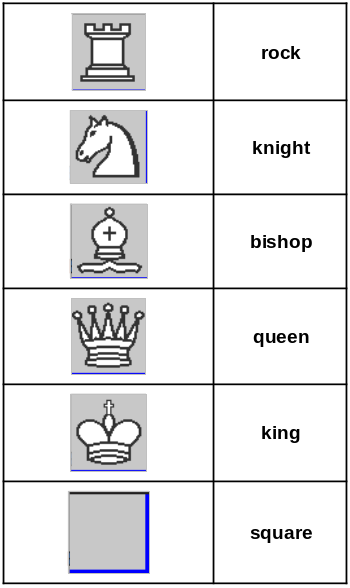
\includegraphics[width=0.3\textwidth,keepaspectratio]{imagenes/picture.png}
	\end{figure}
	
	\begin{itemize}
		\item Estos objetos estarán disponibles importando la biblioteca: \textbf{chessPictures} y estarán internamente representados con arreglos de \textbf{strings} que podrá revisar en el archivo \textbf{pieces.py}
		\item La clase \textbf{Picture} tiene un solo atributo: el arreglo de strings \textbf{img}, el cual contendrá la representación en caracteres de la figura que se desea dibujar.
		\item La clase \textbf{Picture} ya cuenta con una función implementada, no debe modificarla, pero si puede usarla para implementar sus otras funciones.
		\item \textbf{invColor}: recibe un color como un caracter de texto y devuelve su color negativo, también como texto, deberá revisar el archivo colors.py para conocer los valores negativos de cada caracter.
		\item La clase \textbf{Picture} contará además con varios métodos que usted deberá implementar:
		\begin{itemize}
		\item \textbf{verticalMirror:} Devuelve el espejo vertical de la imagen.
		\item \textbf{horizontalMirror:} Devuelve el espejo horizontal de la imagen.
  		\item \textbf{negative:} Devuelve un negativo de la imagen.
  		\item \textbf{join:} Devuelve una nueva figura poniendo la figura del argumento al lado derecho de la figura actual.
		\item \textbf{up:} Devuelve una nueva figura poniendo la figura recibida como argumento, encima de la figura actual.
		\item \textbf{under:} Devuelve una nueva figura poniendo la figura recibida como argumento, sobre la figura actual.
		\item \textbf{horizontalRepeat:} Devuelve una nueva figura repitiendo la figura actual al costado la cantidad de veces que indique el valor de n.
		\item \textbf{verticalRepeat:} Devuelve una nueva figura repitiendo la figura actual debajo, la cantidad de veces que indique el valor de n.
		\end{itemize}
		\item Tenga en cuenta que para implementar todos estos métodos, solo deberá trabajar sobre la representación interna de un    \textbf{Picture}, es decir su atributo \textbf{img}.
		\item Para dibujar una objeto \textbf{Picture} bastará importar el método \textbf{draw} de la biblioteca \textbf{interpreter} y usarlo de la siguiente manera:
	\end{itemize}
	\begin{lstlisting}[style=ascii-tree]
$ python3
Python 3.9.2 (default, Feb 28 2021, 17:03:44)
[GCC 10.2.1 20210110] on linux
Type "help", "copyright", "credits" or "license" for more information.
>>> from chessPictures import *
>>> from interpreter import draw
pygame 1.9.6
Hello from the pygame community. https://www.pygame.org/contribute.html
>>> draw(rock)
3 directories, 20 files
	\end{lstlisting} 
	\begin{figure}[H]
		\centering
		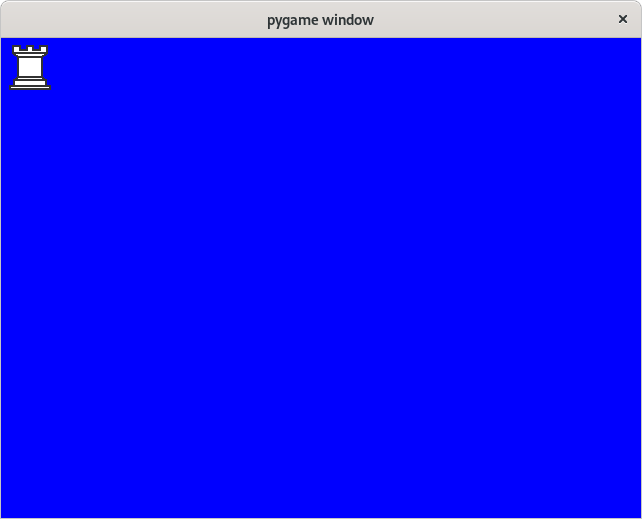
\includegraphics[width=0.3\textwidth,keepaspectratio]{imagenes/pygame_rock.png}
	\end{figure}
	
	\begin{itemize}
		\item Ejercicios:
		\begin{itemize}
			\item Para resolver los siguientes ejercicios solo está permitido usar ciclos, condicionales, definición de listas por comprensión, sublistas, map, join, (+), lambda, zip, append, pop, range.
			\item Implemente los métodos de la clase Picture. Se recomienda que implemente la clase picture por etapas, probando realizar los dibujos que se muestran en la siguiente preguntas.
			\item Usando  únicamente los métodos de los objetos de la clase Picture dibuje las siguientes figuras (invoque a draw).
		\end{itemize}
	\end{itemize}
	\clearpage
	
	\subsection{Ejercicio 1}
	
	\begin{itemize}
		\item Código de ejercicio 1
	\end{itemize}
	\lstinputlisting[language=Python, 		caption={Ejercicio2a.py},numbers=left,]{Tarea-del-Ajedrez/Ejercicio2a.py}
	\begin{itemize}
		\item Captura de la ejecución de ejercicio 1
	\end{itemize}
	\begin{figure}[H]
		\centering
		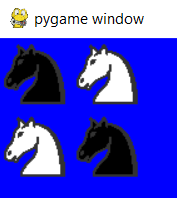
\includegraphics[width=0.3\textwidth,keepaspectratio]{imagenes/ejecucion1.png}
	\end{figure}
	\clearpage
	\subsection{Ejercicio 2}
	
	\begin{itemize}
		\item Código de ejercicio 2
	\end{itemize}
	\lstinputlisting[language=Python, 		caption={Ejercicio2b.py},numbers=left,]{Tarea-del-Ajedrez/Ejercicio2b.py}
	\begin{itemize}
		\item Captura de la ejecución de ejercicio 2
	\end{itemize}
	\begin{figure}[H]
		\centering
		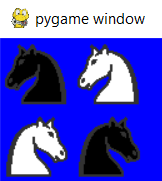
\includegraphics[width=0.3\textwidth,keepaspectratio]{imagenes/ejecucion2.png}
	\end{figure}
	\clearpage
	\subsection{Ejercicio 3}
	
	\begin{itemize}
		\item Código de ejercicio 3
	\end{itemize}
	\lstinputlisting[language=Python, 		caption={Ejercicio2c.py},numbers=left,]{Tarea-del-Ajedrez/Ejercicio2c.py}
	\begin{itemize}
		\item Captura de la ejecución de ejercicio 3
	\end{itemize}
	\begin{figure}[H]
		\centering
		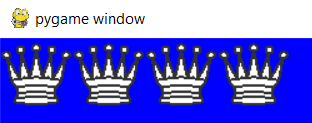
\includegraphics[width=0.6\textwidth,keepaspectratio]{imagenes/ejecucion3.png}
	\end{figure}
	\clearpage
	\subsection{Ejercicio 4}
	
	\begin{itemize}
		\item Código de ejercicio 4
	\end{itemize}
	\lstinputlisting[language=Python, 		caption={Ejercicio2d.py},numbers=left,]{Tarea-del-Ajedrez/Ejercicio2d.py}
	\begin{itemize}
		\item Captura de la ejecución de ejercicio 4
	\end{itemize}
	\begin{figure}[H]
		\centering
		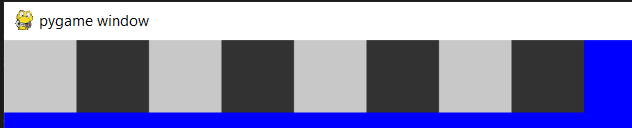
\includegraphics[width=0.6\textwidth,keepaspectratio]{imagenes/ejecucion4.png}
	\end{figure}
	\subsection{Ejercicio 5}
	
	\begin{itemize}
		\item Código de ejercicio 5
	\end{itemize}
	\lstinputlisting[language=Python, 		caption={Ejercicio2e.py},numbers=left,]{Tarea-del-Ajedrez/Ejercicio2e.py}
	\begin{itemize}
		\item Captura de la ejecución de ejercicio 5
	\end{itemize}
	\begin{figure}[H]
		\centering
		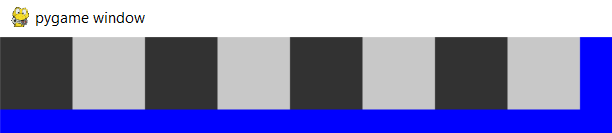
\includegraphics[width=0.6\textwidth,keepaspectratio]{imagenes/ejecucion5.png}
	\end{figure}
	\clearpage
	
	\subsection{Ejercicio 6}
	
	\begin{itemize}
		\item Código de ejercicio 6
	\end{itemize}
	\lstinputlisting[language=Python, 		caption={Ejercicio2f.py},numbers=left,]{Tarea-del-Ajedrez/Ejercicio2f.py}
	\begin{itemize}
		\item Captura de la ejecución de ejercicio 6
	\end{itemize}
	\begin{figure}[H]
		\centering
		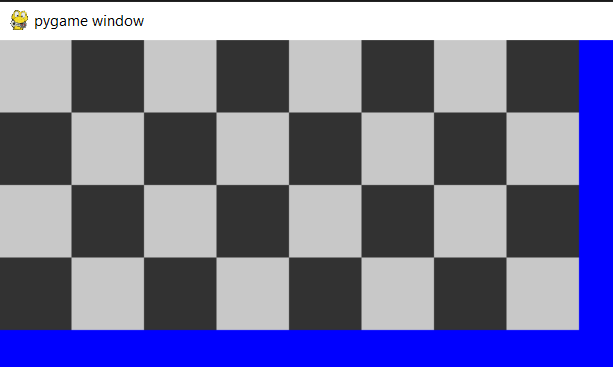
\includegraphics[width=0.5\textwidth,keepaspectratio]{imagenes/ejecucion6.png}
	\end{figure}
	\clearpage
	\subsection{Ejercicio 7}
	
	\begin{itemize}
		\item Código de ejercicio 7
	\end{itemize}
	\lstinputlisting[language=Python, 		caption={Ejercicio2g.py},numbers=left,]{Tarea-del-Ajedrez/Ejercicio2g.py}
	\begin{itemize}
		\item Captura de la ejecución de ejercicio 7
	\end{itemize}
	\begin{figure}[H]
		\centering
		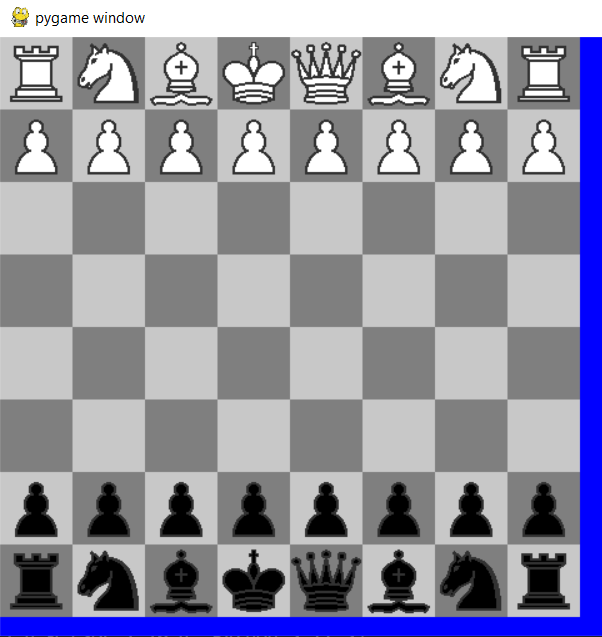
\includegraphics[width=0.5\textwidth,keepaspectratio]{imagenes/ejecucion7.png}
	\end{figure}
	
	\clearpage
	
	\section{Cuestionario}
\begin{itemize}
	\item \textbf{¿Qué son los archivos *.pyc?} \\
		Los archivos *.pyc son archivos de bytecode de Python. Son generados por el intérprete de Python al compilar un archivo fuente *.py. Estos archivos contienen el código fuente de Python compilado en un formato de bajo nivel que puede ser ejecutado más rápidamente por el intérprete de Python.

	\item \textbf{¿Para qué sirve el directorio pycacher?} \\
		El directorio pycache es un directorio utilizado por el intérprete de Python para almacenar archivos de bytecode compilados (*.pyc). Estos archivos se generan automáticamente cuando se importa un módulo en Python. El directorio pycache ayuda a mejorar el rendimiento de la importación de módulos, ya que evita la necesidad de recompilar el código fuente cada vez que se importa un módulo.

	\item \textbf{¿Cuáles son los usos y lo que representa el subguión en Python?} \\
		El subguión en Python tiene varios usos y representaciones dependiendo del contexto:
		\begin{itemize}
			\item Como nombre de variable temporal: Se utiliza cuando no se necesita utilizar el valor de una variable y se desea ignorar. 			
			\item Como nombre de variable "descartable": A veces se utiliza el subguión como nombre de variable cuando el valor no es relevante y solo se necesita ejecutar una función o método. 		
			\item Como nombre de traducción o convención: En algunos casos, se utiliza el subguión como convención para indicar que una variable o método no se utiliza o no es relevante en ese contexto. 
		\end{itemize}
\end{itemize}
	\clearpage
	
	
	\section{\textcolor{red}{Rúbricas}}
	
	\subsection{\textcolor{red}{Entregable Informe}}
	\begin{table}[H]
		\caption{Tipo de Informe}
		\setlength{\tabcolsep}{0.5em} % for the horizontal padding
		{\renewcommand{\arraystretch}{1.5}% for the vertical padding
		\begin{tabular}{|p{3cm}|p{12cm}|}
			\hline
			\multicolumn{2}{|c|}{\textbf{\textcolor{red}{Informe}}}  \\
			\hline 
			\textbf{\textcolor{red}{Latex}} & \textcolor{blue}{El informe está en formato PDF desde Latex,  con un formato limpio (buena presentación) y facil de leer.}   \\ 
			\hline 
			
			
		\end{tabular}
	}
	\end{table}
	
	\clearpage
	
	\subsection{\textcolor{red}{Rúbrica para el contenido del Informe y demostración}}
	\begin{itemize}			
		\item El alumno debe marcar o dejar en blanco en celdas de la columna \textbf{Checklist} si cumplio con el ítem correspondiente.
		\item Si un alumno supera la fecha de entrega,  su calificación será sobre la nota mínima aprobada, siempre y cuando cumpla con todos lo items.
		\item El alumno debe autocalificarse en la columna \textbf{Estudiante} de acuerdo a la siguiente tabla:
	
		\begin{table}[ht]
			\caption{Niveles de desempeño}
			\begin{center}
			\begin{tabular}{ccccc}
    			\hline
    			 & \multicolumn{4}{c}{Nivel}\\
    			\cline{1-5}
    			\textbf{Puntos} & Insatisfactorio 25\%& En Proceso 50\% & Satisfactorio 75\% & Sobresaliente 100\%\\
    			\textbf{2.0}&0.5&1.0&1.5&2.0\\
    			\textbf{4.0}&1.0&2.0&3.0&4.0\\
    		\hline
			\end{tabular}
		\end{center}
	\end{table}	
	
	\end{itemize}
	
	\begin{table}[H]
		\caption{Rúbrica para contenido del Informe y demostración}
		\setlength{\tabcolsep}{0.5em} % for the horizontal padding
		{\renewcommand{\arraystretch}{1.5}% for the vertical padding
		%\begin{center}
		\begin{tabular}{|p{2.7cm}|p{7cm}|x{1.3cm}|p{1.2cm}|p{1.5cm}|p{1.1cm}|}
			\hline
    		\multicolumn{2}{|c|}{Contenido y demostración} & Puntos & Checklist & Estudiante & Profesor\\
			\hline
			\textbf{1. GitHub} & Hay enlace URL activo del directorio para el  laboratorio hacia su repositorio GitHub con código fuente terminado y fácil de revisar. &2 &X &2 & \\ 
			\hline
			\textbf{2. Commits} &  Hay capturas de pantalla de los commits más importantes con sus explicaciones detalladas. (El profesor puede preguntar para refrendar calificación). &4 & & & \\ 
			\hline 
			\textbf{3. Código fuente} &  Hay porciones de código fuente importantes con numeración y explicaciones detalladas de sus funciones. &2 &X &2 & \\ 
			\hline 
			\textbf{4. Ejecución} & Se incluyen ejecuciones/pruebas del código fuente  explicadas gradualmente. &2 &X &2 & \\ 
			\hline			
			\textbf{5. Pregunta} & Se responde con completitud a la pregunta formulada en la tarea.  (El profesor puede preguntar para refrendar calificación).  &2 &X &2 & \\ 
			\hline	
			\textbf{6. Fechas} & Las fechas de modificación del código fuente estan dentro de los plazos de fecha de entrega establecidos. &2 &X &2 & \\ 
			\hline 
			\textbf{7. Ortografía} & El documento no muestra errores ortográficos. &2 &X &2 & \\ 
			\hline 
			\textbf{8. Madurez} & El Informe muestra de manera general una evolución de la madurez del código fuente,  explicaciones puntuales pero precisas y un acabado impecable.   (El profesor puede preguntar para refrendar calificación).  &4 & & & \\ 
			\hline
			\multicolumn{2}{|c|}{\textbf{Total}} &20 & &12 & \\ 
			\hline
		\end{tabular}
		%\end{center}
		%\label{tab:multicol}
		}
	\end{table}
	
\clearpage

\section{Referencias}
\begin{itemize}			
	\item \url{https://www.w3schools.com/java/default.asp}
	\item \url{https://www.geeksforgeeks.org/insertion-sort/}
\end{itemize}	
	
%\clearpage
%\bibliographystyle{apalike}
%\bibliographystyle{IEEEtranN}
%\bibliography{bibliography}
			
\end{document}